\documentclass[12pt,a4paper]{article}

% Paquetes básicos
\usepackage[utf8]{inputenc}
\usepackage[spanish]{babel}
\usepackage{graphicx}
\usepackage{amsmath}
\usepackage{hyperref}
\usepackage{float}
\usepackage{subcaption}
\usepackage{listings}
\usepackage{xcolor}
\usepackage{geometry}
\usepackage{booktabs}

% Configuración de márgenes
\geometry{
    left=2.5cm,
    right=2.5cm,
    top=2.5cm,
    bottom=2.5cm
}

% Configuración de código
\lstset{
    language=Python,
    basicstyle=\ttfamily\small,
    keywordstyle=\color{blue},
    commentstyle=\color{gray},
    stringstyle=\color{red},
    numbers=left,
    numberstyle=\tiny\color{gray},
    breaklines=true,
    frame=single,
    captionpos=b
}

% Información del documento
\title{\textbf{Práctica 01: Aprendizaje por Refuerzo}}
\author{
    Pablo Chantada Saborido -
    \texttt{pablo.chantada@udc.es}\\
    Laura Cabaleiro Pintos -
    \texttt{laura.cabaleiro.pintos@udc.es}\\
    Robótica Inteligente Aplicada\\
    Universidad de A Coruña
}

\begin{document}

\maketitle

\section{Definición del Problema}

\subsection{Espacio de Observaciones}

El espacio de observaciones es \textbf{continuo} (8 dimensiones) y contiene:

\begin{table}[H]
\centering
\begin{tabular}{@{}lll@{}}
\toprule
\textbf{Variable} & \textbf{Rango} & \textbf{Descripción} \\ \midrule
Posición agente (x, z) & [-1, 1] & Posición normalizada del robot \\
Posición objetivo (x, z) & [-1, 1] & Posición normalizada del cilindro \\
Blob visible & \{0, 1\} & Visibilidad del cilindro en cámara \\
Posición blob (x, y) & [-1, 1] & Posición del blob en cámara \\
Tamaño blob & [0, 1] & Tamaño del blob (distancia) \\ \bottomrule
\end{tabular}
\caption{Elementos del espacio de observaciones}
\end{table}

\textbf{Justificación:} Se utiliza espacio continuo para mayor precisión y se combinan datos de posicionamiento absoluto (posiciones de los elementos) con información visual.

\subsection{Espacio de Acciones}

Espacio \textbf{continuo} bidimensional:
\begin{equation}
\mathbf{a} = [v_{\text{left}}, v_{\text{right}}]
\end{equation}

donde $v_{\text{left}}$ y $v_{\text{right}}$ son las velocidades normalizadas de las ruedas izquierda y derecha.

\textbf{Escalado al motor:} Las acciones se transforman mediante:
\begin{equation}
v_{\text{motor}} = \text{clip}(v_{\text{norm}} \times S, -100, 100)
\end{equation}

resultando en un rango efectivo de $[-S, S]$, donde $S$ indica la velocidad máxima de las ruedas ($[-20, 20]$). 

\textbf{Justificación:} Las acciones continuas permiten movimientos suaves y precisos. El factor de escala ($S$) proporciona control y estabilidad.


\subsection{Función de Recompensa}

La función de recompensa combina múltiples componentes:

\begin{equation}
R_t = R_{\text{dist}} + R_{\text{vis}} + R_{\text{goal}}
\end{equation}

Donde:

\begin{itemize}
    \item \textbf{Recompensa por distancia} ($R_{\text{dist}}$):
    \begin{equation}
    R_{\text{dist}} = 0.05 \times (d_{t-1} - d_t)
    \end{equation}
    
    \item \textbf{Recompensa por visibilidad} ($R_{\text{vis}}$):
    \begin{align}
    R_{\text{vis}} = \begin{cases}
    0.2 + 0.2 \times (1 - \frac{|x_{\text{blob}} - 50|}{50}) + 0.1 \times \frac{\text{size}_{\text{blob}}}{400} & \text{si visible} \\
    -0.15 & \text{si no visible}
    \end{cases}
    \end{align}
    Recompensa por mantener el blob visible y centrado, teniendo en cuenta su tamaño.
    
    \item \textbf{Recompensa por objetivo alcanzado} ($R_{\text{goal}}$):
    \begin{equation}
    R_{\text{goal}} = \begin{cases}
    10.0 & \text{si } d_t < 150 \\
    0 & \text{en otro caso}
    \end{cases}
    \end{equation}
\end{itemize}

\textbf{Justificación:} Esta recompensa, basada en múltiples aspectos (visión, cámara, tamaño del blob, etc.), permite al agente explotar al máximo el espacio de observación, proporcionando una señal de recompensa mucho más rica y realista que usar únicamente la distancia absoluta.

\section{Implementación}

\subsection{Algoritmo de Aprendizaje: SAC}

Se seleccionó \textbf{Soft Actor-Critic (SAC)}\footnote{Aún no habíamos llegado a la teoría de SAC.} por un mejor rendimiento en comparación con otros modelos, principalmente PPO y DQN. Este mejor rendimiento se obtuvo a través de prueba y error con iteraciones básicas. Es muy posible que otros algoritmos obtengan un rendimiento similar o superior.

\subsection{Hiperparámetros}

\begin{table}[H]
\centering
\begin{tabular}{@{}ll@{}}
\toprule
\textbf{Parámetro} & \textbf{Valor} \\ \midrule
Algoritmo & SAC \\
Learning rate & 3e-4 \\
Gamma (factor de descuento) & 0.95 \\
Buffer size & 2,000 \\
Batch size & 64 \\
Tau (soft update) & 0.005 \\
Learning starts & 500 \\
Train frequency & 2 \\
Gradient steps & 2 \\
Entropy coefficient & auto \\
Episodios Fase 1 & 234 \\
Episodios Fase 2 & 100 \\
Pasos por episodio & 30 \\
\textbf{Total timesteps} & \textbf{10,020} \\ \bottomrule
\end{tabular}
\caption{Configuración de hiperparámetros}
\end{table}

\subsection{Arquitectura del Sistema}

El sistema consta de tres componentes principales:

\begin{enumerate}
    \item \textbf{Environment} (\texttt{env.py}): Implementa \texttt{gym.Env}
    \item \textbf{Training} (\texttt{train.py}): Entrenamiento con callbacks
    \item \textbf{Evaluation} (\texttt{eval.py}): Validación del modelo
\end{enumerate}

\subsection{Características Especiales}

El entrenamiento se divide en dos fases. En la Fase 1 (234 episodios), el cilindro permanece estático para que el agente aprenda comportamientos básicos. En la Fase 2 (100 episodios), el cilindro se mueve de manera continua con trayectorias curvas.

\setlength{\parskip}{0.5em}

\textbf{Normalización:} Todas las observaciones están normalizadas en rangos [-1, 1] o [0, 1] para facilitar el aprendizaje.

\section{Resultados Experimentales} 

\subsection{Métricas de Entrenamiento}


\begin{figure}[H]
    \centering
    \begin{subfigure}[t]{0.48\textwidth}
        \centering
        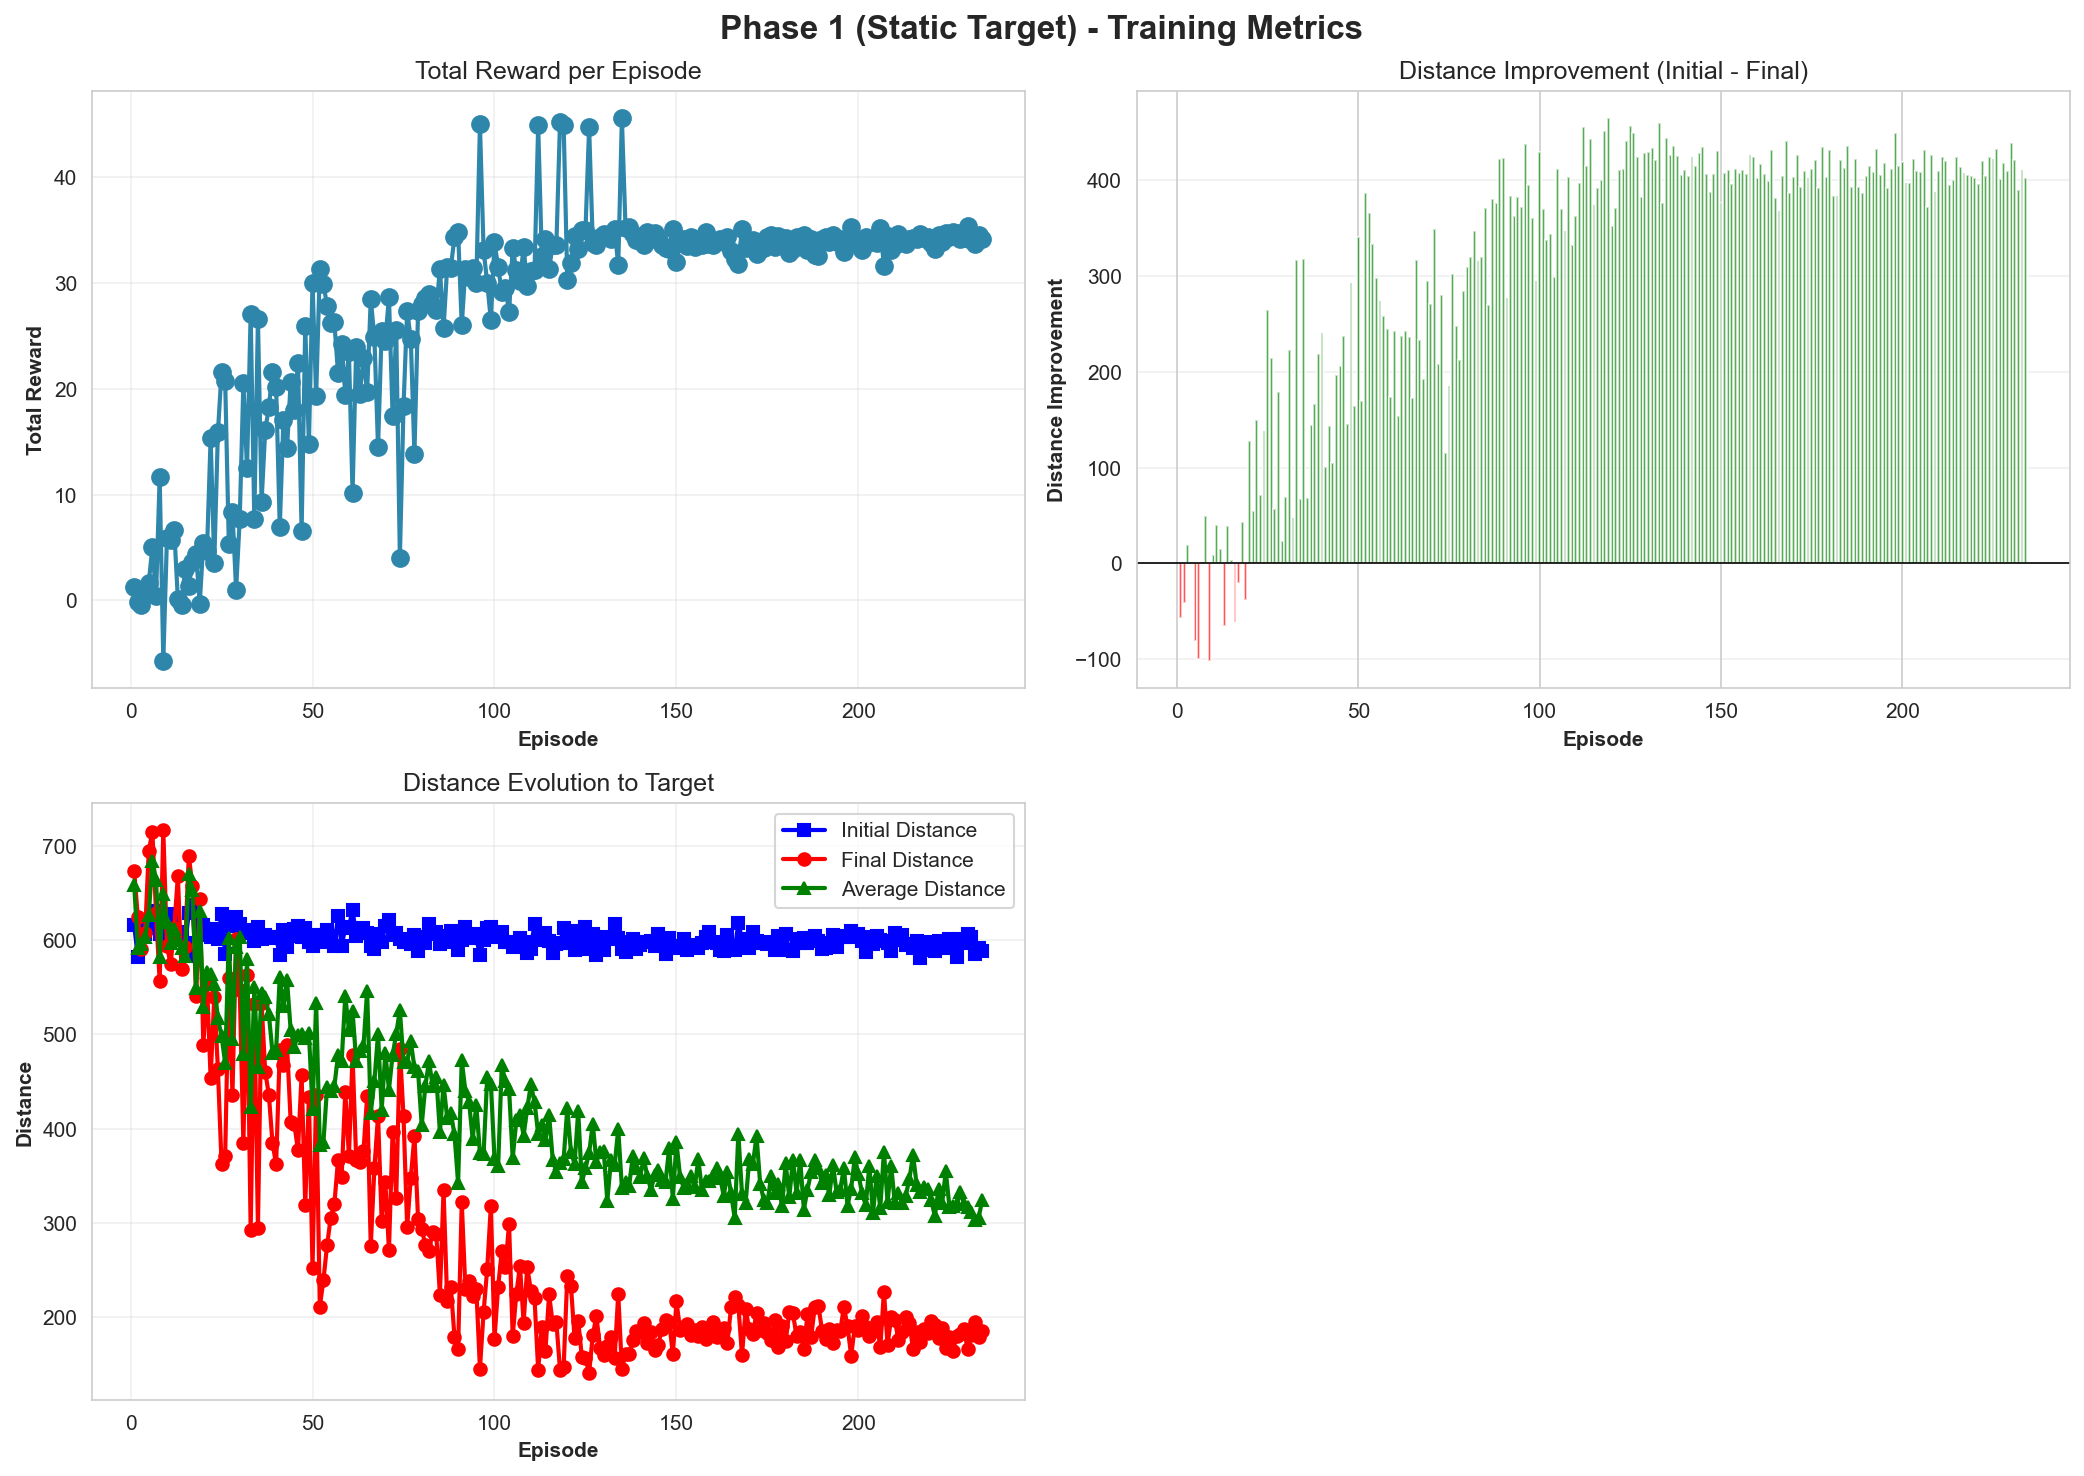
\includegraphics[width=\textwidth]{logs/episode_metrics_phase1.png}
        \caption{Fase 1: objetivo estático.}
        \label{fig:metrics_phase1}
    \end{subfigure}
    \hfill
    \begin{subfigure}[t]{0.48\textwidth}
        \centering
        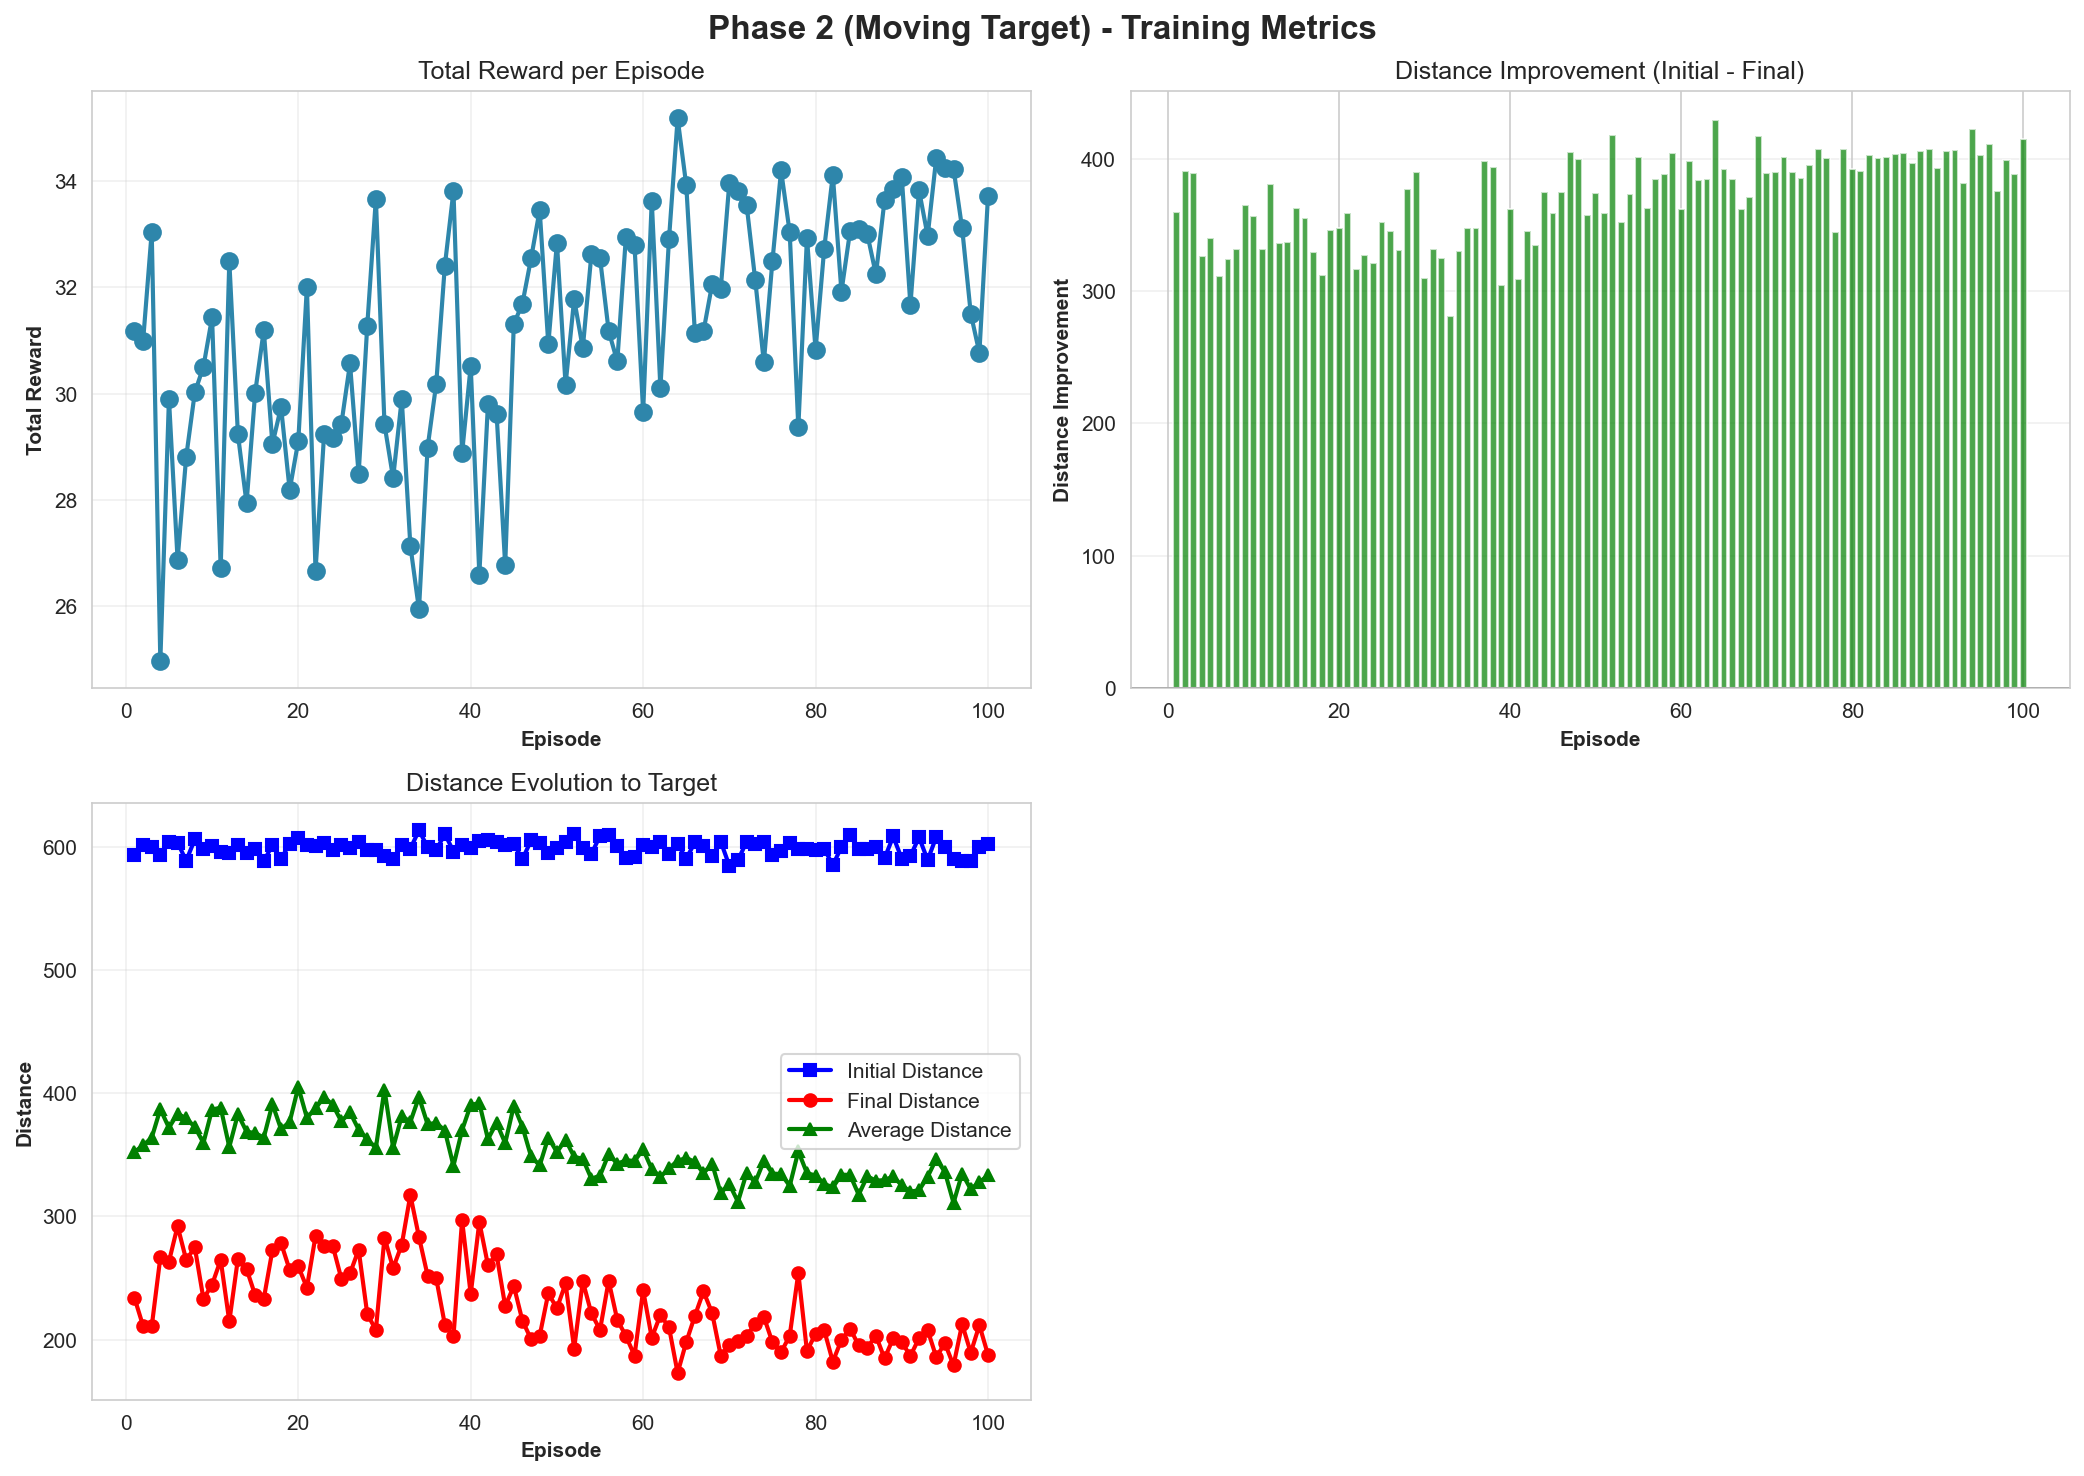
\includegraphics[width=\textwidth]{logs/episode_metrics_phase2.png}
        \caption{Fase 2: objetivo móvil.}
        \label{fig:metrics_phase2}
    \end{subfigure}
    \caption{Evolución de las métricas de entrenamiento en ambas fases. Se observa una transición desde un comportamiento irregular hacia un aprendizaje estable y consistente.}
    \label{fig:training_metrics_comparison}
\end{figure}


\textbf{Análisis:}

En la \textbf{Fase 1} se observa un comportamiento irregular, con episodios en los que la mejora de la distancia es negativa. En la \textbf{Fase 2}, el rendimiento se vuelve más estable, evidenciando un aprendizaje efectivo.

La \textbf{recompensa media} aumenta progresivamente, con ligeras caídas tras los reinicios de los episodios, mientras que la \textbf{distancia final al objetivo} disminuye de forma constante, indicando que el agente mejora su capacidad para alcanzar el objetivo en menos pasos.


\subsection{Trayectorias 2D}

\begin{figure}[H]
    \centering
    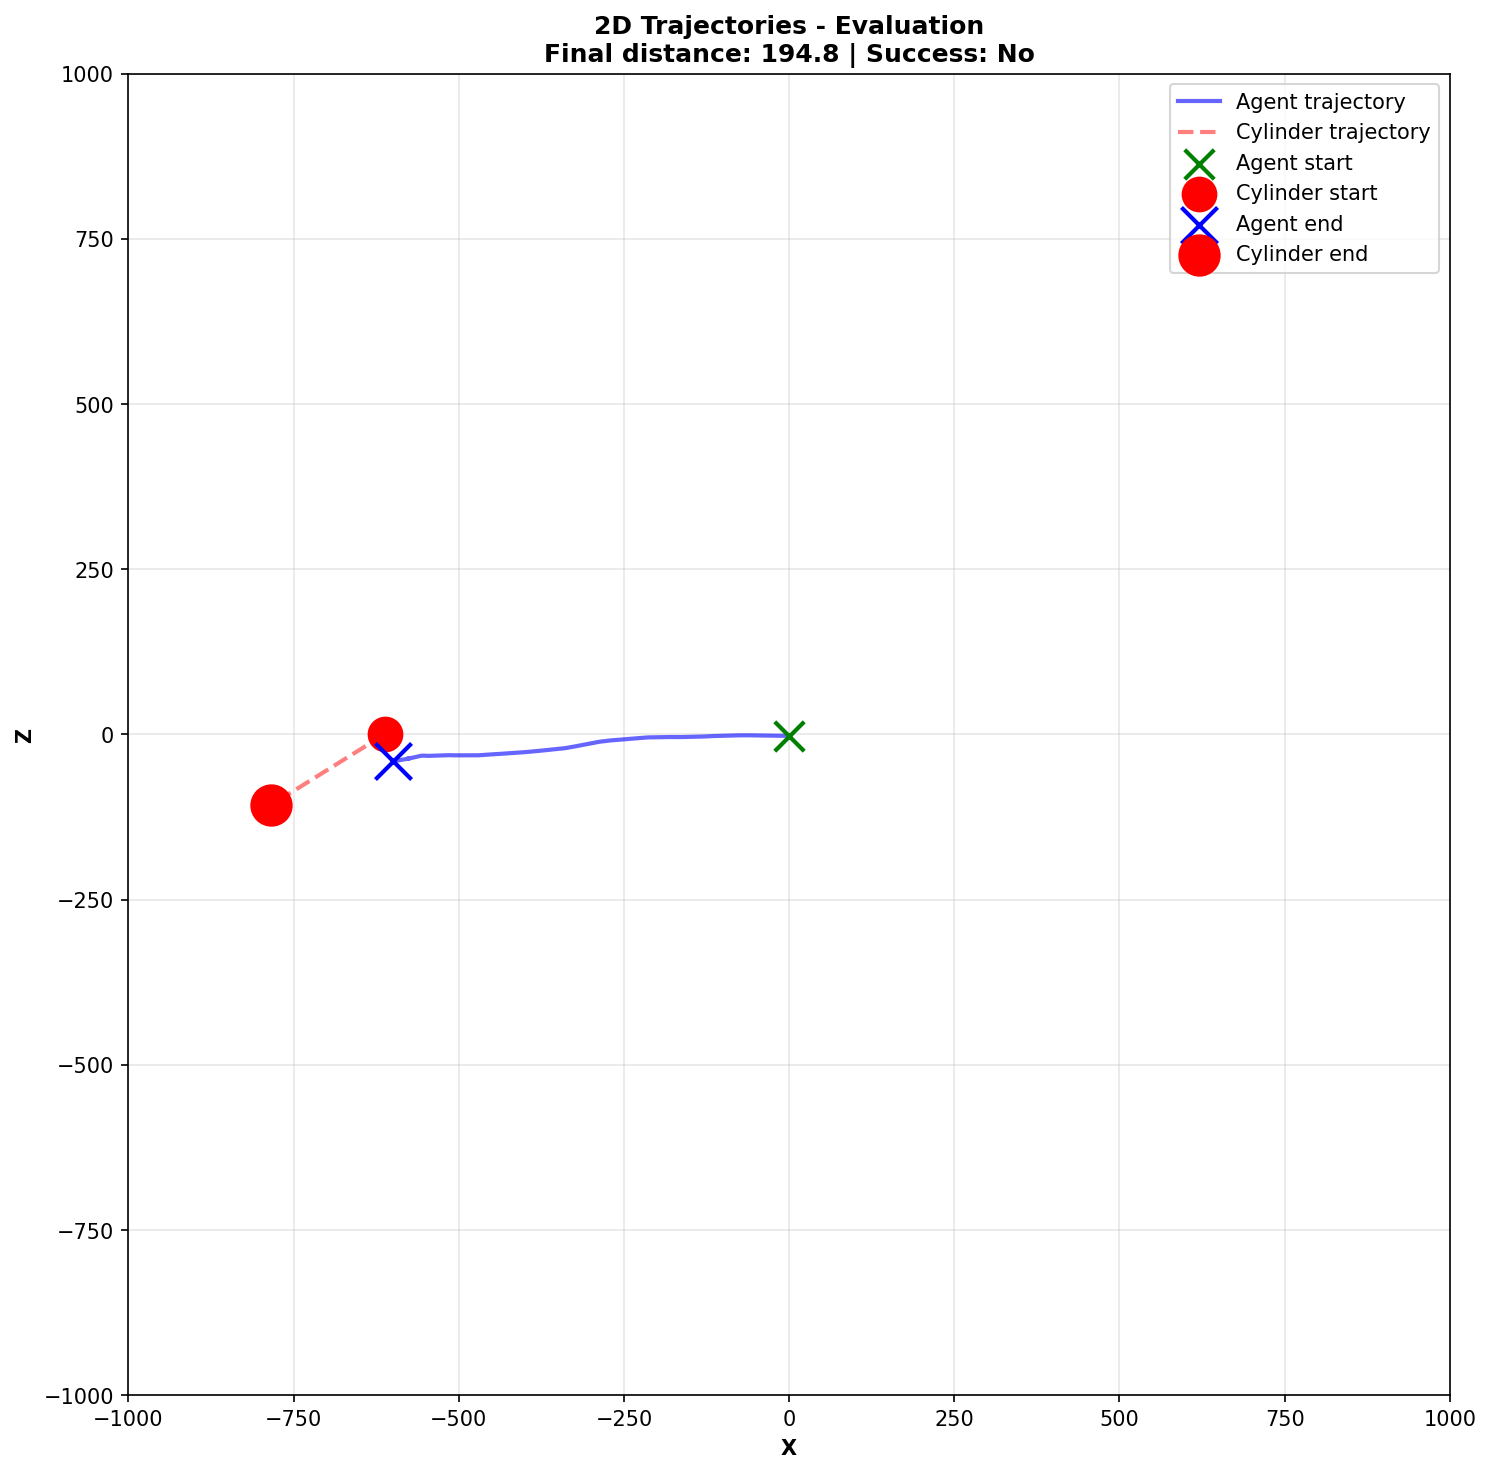
\includegraphics[width=0.4\textwidth]{logs/evaluation_trajectory.png}
    \caption{Trayectoria del agente (azul) siguiendo el cilindro móvil (rojo). Los marcadores indican posiciones de inicio y fin.}
    \label{fig:trajectories}
\end{figure}


\subsection{Rendimiento del Sistema}

\begin{table}[H]
\centering
\begin{tabular}{@{}lc@{}}
\toprule
\textbf{Métrica} & \textbf{Valor} \\ \midrule
Pasos para convergencia Fase 1 & $\sim$4,500 \\
Recompensa media Fase 1 & +2.5 a +4.0 \\
Recompensa media Fase 2 & +1.5 a +3.0 \\
Tiempo de entrenamiento & $\sim$45-60 min \\ \bottomrule
\end{tabular}
\caption{Métricas de rendimiento del sistema}
\end{table}

\section{Conclusiones}

El robot obtiene un rendimiento correcto y rápido, demostrando la capacidad de adaptación del \textbf{Aprendizaje por Refuerzo} a nuevos entornos. Además, se observa el valor de la normalización y discretización de los espacios gracias al esquema obtenido de Gymnasium. Si bien puede ser un algoritmo insuficiente para tareas más complejas, demuestra su valor en entornos relativamente reales.

\end{document}
